\section*{Conclusione}

Per quanto riguarda lo Slew Rate del nostro amplificatore operazioanle abbiamo ottenuto che ha un valore di $SR_s\,=\,(0.498\,\pm\,0.004)\,\frac{\SI{}{\volt}}{\SI{}{\micro\second}}$ per il fronte d'onda in salita, mentre di $SR_d\,=\,(-0.353\,\pm\,0.003)\,\frac{\SI{}{\volt}}{\SI{}{\micro\second}}$ per il fronte d'onda in discesa. Confrontando i dati ottenui con quelli del costruttore, che fornisce un valore dello Slew Rate di $0.5 \frac{\SI{}{\volt}}{\SI{}{\micro\second}}$ possaimo dire che i valori da noi ottenuti sono corretti. Questo è vero in quanto il valore dello Slew Rate di salita è compatibile col valore fornitoci dal costruttore. Infine possiamo presupporre che i due ritardi non sono uguali, ma quello della salita è minore di quelo di discesa, in quanto il tempo caratteristico di carica del condensatore sia minore di quello di scarica dello stesso. Questo probabilmete porta ad una risposta più lenta dell'amplificatore ai fronti d'onda in discesa che in salita.

A riguardo della corrente massima che il nostro amplificatore operazionale può erogare possiamo solo dire che il valore da noi trovato $I\ped{max}\,=\,(13.5\,\pm\,0.7)\,\SI{}{\milli\ampere}$ è compreso all'interno del range fornitoci dal costruttore. Tale range comprende valori che vanno da $\pm10$ a $\pm20$ $\SI{}{\milli\ampere}$.

Anche per quanto riguarda i range di valori di frequanza che permettono di mantenere un guadagno costate dell'OPAMP possiamo dire che quelli trovati sono compatibili con quelli forniti dal costruttore. Come è possibile osservare dai grafici in Figura \ref{fig:DB_plot} il guadagno dell'amplificatore operazionale diminuisce man mano che le frequenze aumentano fino quasi a diventare unitario per frequenze che si aggirano attorno ai $\SI{}{\mega\hertz}$.

Per concludere possimo dire che il grafico ottenuto (Figura \ref{fig:G_openloop_plot1}) relativo al guadagno $G$ dell'amplificatore operazionale in configurazione open loop è simole a quello fornitoci dal costruttore. Pertanto possiamo concludere che con quest'ultima verifica abbiamo discusso tutte le caratteristiche che differenziano un OPAMP ideale da uno reale e abbiamo anche verificato che le specifiche tecniche fornitci dal costruttore sono corrette e trovano riscontro con l'analisi sperimentale.

\begin{figure}[h]
\centering
    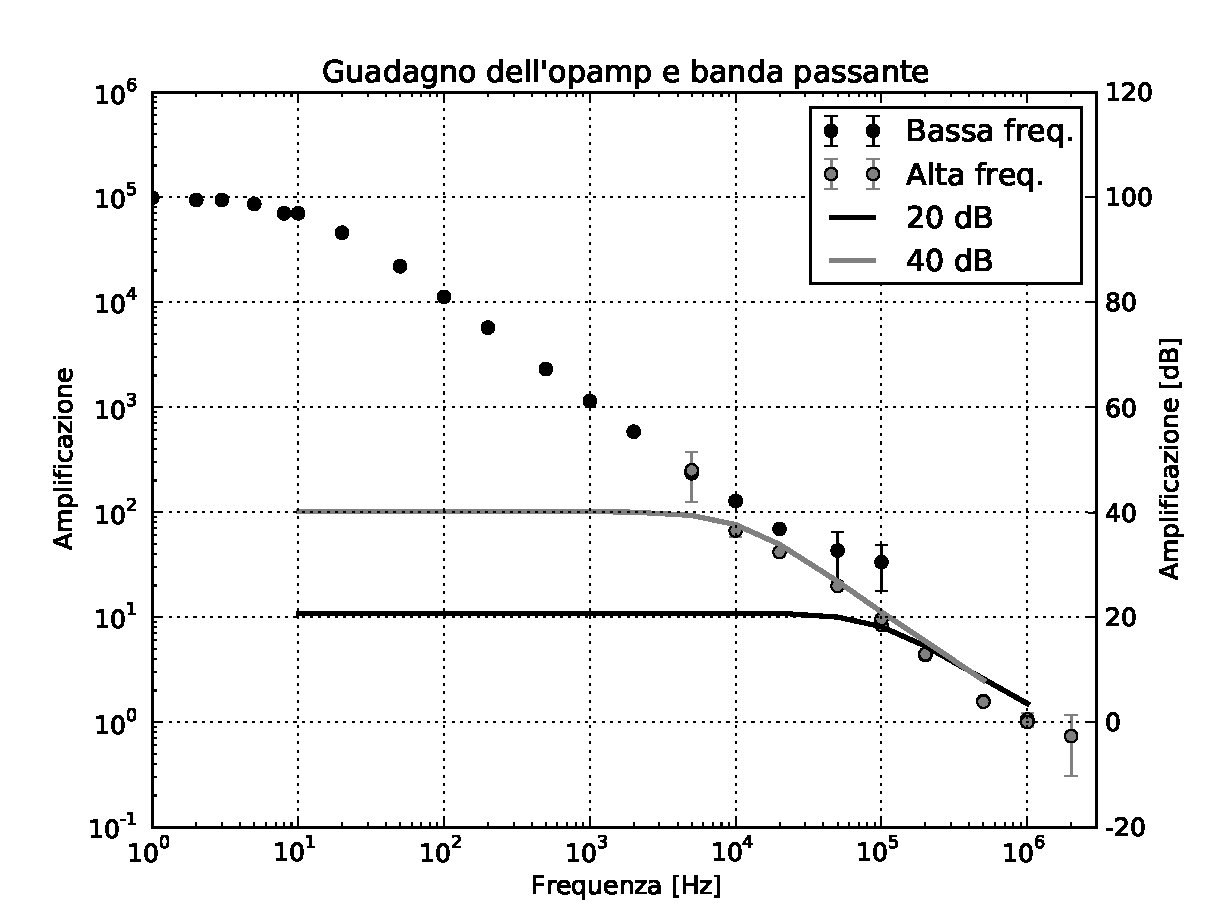
\includegraphics[width=0.7\textwidth]{Figure/gabp.pdf}
    \caption{Nel grafico sono visibili gli stessi dati delle Figure \ref{fig:DB_plot} e \ref{fig:G_openloop_plot1}. Come si può notare è proprio a causa dell'andamento del guadagno in funzione della frequenza dell'OPAMP che questi circuiti hanno una frequenza di taglio ed una riduzione del guadagno. Come riportato nella didascalia la linea grigia mostra l'andamento del guadagno del circuito (Figura \ref{fig:banda_passante}) con $G$ ideale di 20 dB, mentre la linea nera è relativa ad un guadagno ideale $G$ di 40 dB. Per la discussione sulle incertezze di misura si rimanda alla discussione fatta per il grafico in Figura \ref{fig:G_openloop_plot1}.}
    \label{fig:G_openloop_plot2}
\end{figure}
